%%%%%%%%%%%%%%%%%%%%%%%%%%%%%%%%%%%%%%%%%%%%%%%%%%%%%%%%%%%%%%%%%%%%%%%
%
% Dissertationen mit LaTeX auf dem edoc-Server
%
% Humboldt-Universitaet zu Berlin
% Computer- und Medienservice
% Arbeitsgruppe Elektronisches Publizieren
% Bezug der Vorlage und der Richtlinien:
%     http://edoc.hu-berlin.de/e_autoren/latex/
%
% Kontakt:
%     E-Mail:
%                   edoc-latex@rz.hu-berlin.de
%     Telefon:              siehe
%     http://edoc.hu-berlin.de/e_autoren/latex/kontakt.php  %
%
%%%%%%%%%%%%%%%%%%%%%%%%%%%%%%%%%%%%%%%%%%%%%%%%%%%%%%%%%%%%%%%%%%%%%%%
%                                                                     %
% Das folgende Template muss f�r die Publikation von digitalen        %
% Dissertationen in LaTeX an der Humboldt-Universit�t benutzt werden. %
%                                                                     %
% Aendern Sie den Name dieser Datei auf ihren_nachname.tex.           %
%                                                                     %
% Die mit einem Stern (*) gekennzeichnete Teile sind optional;        %
% falls Sie sie nicht verwenden m�chten, sind entsprechende Zeile     %
% zu entfernen.                                                       %
%                                                                     %
%%%%%%%%%%%%%%%%%%%%%%%%%%%%%%%%%%%%%%%%%%%%%%%%%%%%%%%%%%%%%%%%%%%%%%%

% \listfiles    % Erstellt eine Liste von allen benutzten Dateien
% zusammen mit ihrer Versionen
% und ggf. einer kurzen Beschreibung
% Sie wird in die log-Datei geschrieben

%\documentclass[12pt,a4paper% die Verwendung von DIN-A4-Format ist pflicht!
\documentclass[pdftex,a4paper]{scrreprt}
\usepackage[top=2cm, bottom=2cm, left=2cm, right=2cm]{geometry}

%notwendige Pakete
%\usepackage[ngerman, english]{babel}    % mehrsprachiger Textsatz
\usepackage[english, ngerman]{babel}    % mehrsprachiger Textsatz
% babel: letzte Sprache in Optionen zeigt die Sprache des Dokumentes
% und kann durch den Befehl \selectlanguage{} geaendert werden
% Passen Sie die Optionen des babel-Paketes nach Bedarf an!
\usepackage[utf8]{inputenc}       % Eingabekodierung Parameter latin1 darf ge�ndert werden
\usepackage[T1]{fontenc}                % Schriftenkodierung
\usepackage{graphicx}                       % zum Einbinden von Grafiken
\usepackage{lmodern}                        % Ersatz fuer Computer Modern-Schriften
                                                                % zum besseren Aussehen am Bildschirm
                                                                
%-Eingabe der Metadaten des Titelblattes--------------------------

%-Daten des Autors / Authors Data---------------------------------

\newcommand{\dcauthorpre}{Herrn} 
\newcommand{\dcauthorsurname}{Krieg} 
\newcommand{\dcauthorname}{Jan-Lukas} 
\newcommand{\dcauthoradd}{geboren am 09.01.1995 in Berlin}

%-Titel und Untertitel / Title and subtitle-----------------------

\newcommand{\dctitle}{Untersuchungen zur Ausrichtung einer CCD-Kamera am MST-Prototyp} 
\newcommand{\dcsubtitle}{~}  
% Falls dcsubtitle NICHT verwendet werden soll, {\dcsubtitle}{~} eingeben.

%-Eingabe der Betreuuernahmen / Names of the consultants---------

\newcommand{\dcconsulta}{Dr. Ullrich Schwanke} 
%\newcommand{\dcconsultb}{Priv.-Doz. Dr. K. Hennig} 

%-Eingabe der Gutachternamen / Names of the approvals-------------

\newcommand{\dcapprovala}{Prof. Dr. Thomas Lohse} 
\newcommand{\dcapprovalb}{Prof. Dr. David Berge} 
%\newcommand{\dcapprovalc}{Prof. Dr. Elsa Brandt} 

%-Information zur Universitaet------------------------------------

\newcommand{\dcdegree}{Bachelor of Science\\(B. Sc.)} 
\newcommand{\dcsubject}{Physik} 
\newcommand{\dcfaculty}{Mathematisch-Naturwissenschaftlichen Fakult\"at}
\newcommand{\dcinstitute}{Institut f\"ur Physik}
\newcommand{\dcuniversity}{Humboldt-Universit\"at zu Berlin}
\newcommand{\dcdean}{Prof. Dr. Elmar Kulke}
\newcommand{\dcpresident}{Prof. Dr.-Ing. Sabine Kunst}

%-Pruefungsdaten: eingereicht und mdl. Pruefung-------------------
%-data of submission and oral exam--------------------------------

\newcommand{\dcdatesubmitted}{1. M�rz 2019} %auch wenn nicht auf dem Titelblatt, bitte erf�llen!
\newcommand{\dcdateexam}{1. M�rz 2019} 

%-deutsche Schlagwoerter / german keywords------------------------

\newcommand{\dckeydea}{CTA}
\newcommand{\dckeydeb}{MST-Prototyop}
\newcommand{\dckeydec}{Adlershof}
\newcommand{\dckeyded}{Pointing}

% Folgende Zeile bitte nicht aendern!
\newcommand{\dckeywordsde}{\vfill \raggedright {\textbf{Schlagw\"orter:}}\\ \dckeydea, \dckeydeb, \dckeydec, \dckeyded \\}

%-englische Schlagwoerter / english keywords----------------------

\newcommand{\dckeyena}{keyword 1}
\newcommand{\dckeyenb}{keyword 2}
\newcommand{\dckeyenc}{keyword 3}
\newcommand{\dckeyend}{keyword 4}

% Folgende Zeile bitte nicht aendern!
\newcommand{\dckeywordsen}{\vfill \raggedright {\textbf{Keywords:}}\\ \dckeyena, \dckeyenb, \dckeyenc, \dckeyend \\}

\newcommand{\dcpdfsubject}{Dissertation}
                          % Bitte ALLE Angaben erf�llen!
\usepackage{ifpdf}

\ifpdf
%%das kann man benutzen, wenn man andere Formate benutzen will
%\DeclareGraphicsExtensions{{.pdf}}   %Endung der Grafiken, wenn nicht pdf
% die folgenden Angaben sind im PDF unter Datei | Dokumenteigenschaften 
% in Acrobat / Acrobat Reader sichtbar
% Aendern Sie bitte die Daten, wo noetig!
\usepackage[%
	pdftitle={\dctitle},
	pdfauthor={\dcauthorsurname\ \dcauthorname},
	pdfsubject={\dcpdfsubject}, % optional
	pdfkeywords={\dckeydea, \dckeydeb, \dckeydec, \dckeyded},
	pdfpagemode=UseOutlines,
  colorlinks=true,					% bitte nicht �ndern!
	linkcolor=black,					% bitte nicht �ndern!
	filecolor=black,					% bitte nicht �ndern!
	urlcolor=black,						% bitte nicht �ndern!
	citecolor=black,					% bitte nicht �ndern!
	pdftex=true,              % bitte nicht �ndern!
	plainpages=false,         % bitte nicht �ndern!
	hypertexnames=false,      % bitte nicht �ndern!
	pdfpagelabels=true,       % bitte nicht �ndern!
	hyperindex=true]{hyperref}% bitte nicht �ndern!
\else
  % hier kann mann eventuelle Befehle umdefinieren
  % die nur f�r pdfLaTeX vorgesehen sind
  % und das richtige Kompilieren durch den normalen LaTeX verhindern
	\newcommand{\texorpdfstring}[1]{#1}
\fi

%-Eigene Trennregeln*---------------------------------------------

% % Tragen Sie Ihre eigenen Trennregel ein:
\hyphenation{Bei-spiel, �-ko-lo-gie}

%-zusaetzliche Kommandos*-----------------------------------------
%\titleformat{\chapter}[hang]{\Huge\bfseries}{\thechapter\hsp\textcolor{gray75}{|}\hsp}{0pt}{\Huge\bfseries}
%\renewcommand{\chaptername}{}

%\renewcommand{\thechapter}{}
%\include{command}
\include{amsmath}
%eigene Pakete
\usepackage{units}
\usepackage{isotope}
\usepackage{booktabs}

%-Dokument--------------------------------------------------------

\begin{document}
% Es muss zitiert werden k�nnen! Im Vorspann roemisch,
% Im Hauptteil benutzt man arabische Nummerierung.
\pagenumbering{roman}

%-Titelblatt------------------------------------------------------

%----------Generierung der Titelseite-----bitte nicht ver�ndern!--------------------


\author{von \\ \dcauthorpre\ \dcauthorname\ \dcauthorsurname\ \\ \dcauthoradd}

%----------
\title{ \vspace{-2cm}\dctitle \\ 
\vspace{0.5cm}
\large{\dcsubtitle} \\ 
\vspace{0.5cm} {\Large{BACHELORARBEIT}}\\ 
\vspace{0.5cm} \large{zur Erlangung des akademischen Grades \\ 
\dcdegree\\ im Fach \dcsubject \\\vspace{0.5cm}

\includegraphics[width=6cm]{husiegel}\\ 
\vspace{0.5cm} eingereicht an der \\ 
\dcfaculty \\ 
\dcinstitute\\
\dcuniversity \\}}
%-----------------
\date{\vspace{2.5cm}
%\raggedright{
%Pr\"asident der Humboldt-Universit\"at zu Berlin:\\
%\dcpresident \vspace{-0.3cm}
%}\vspace{0.5cm}\\
%
%\raggedright{
%Dekan der \dcfaculty:\\
%\dcdean \vspace{-0.3cm}
%}\vspace{0.5cm}\\
%
% auskommentiert weil nicht standard
\vspace{-1cm}
\raggedright{
Gutachter:
\begin{enumerate} 
\item{\it\dcapprovala} \vspace{-0.2cm}
\item{\it\dcapprovalb} \vspace{-0.2cm}
%\item{\it\dcapprovalc} \vspace{-0.3cm}
\end{enumerate}} \vspace{0.5cm}
\raggedright{
Betreuung:
\begin{enumerate} 
\item{\it\dcconsulta} \vspace{-0.2cm}
%\item{\it\dcconsultb} \vspace{-0.2cm}
\end{enumerate}} \vspace{0.5cm}
%-----------------
\raggedright{
\begin{tabular}{lll}
eingereicht am: &  &\it\dcdatesubmitted\\ % wenn nicht in der Pr�fungsordnung, die Zeile bitte auskommentieren
%Tag der m\"undlichen Pr\"ufung: & & \dcdateexam
\end{tabular}}\\ 
}
%-------------------------------------                         % Bitte KEINE �nderungen vornehmen!
\maketitle
%-englische-Zusammenfassung---------------------------------------
%
%\selectlanguage{english}
%
%\begin{abstract}
%\setcounter{page}{2} % Nach Bedarf anpassen!
%Here is the english abstract.\\
%% hier werden die englische Schlagw�rter aus Metadaten �bernommen
%\dckeywordsen				
%\end{abstract}

%-deutsche Zusammenfassung----------------------------------------

%\selectlanguage{german}

\begin{abstract}
%\setcounter{page}{3} % Nach Bedarf anpassen!
%Das CTA ist ein internationales Projekt, dass die aktuelle Generation an Tscherenkow-Teleskopen ersetzen soll. F\"ur eines der Teleskope in Berlin ein Prototyp errichtet, um den Aufbau und die Funktion zu testen. Um das Pointing zu testen befinden sich im Zentrum des Reflektors drei CCD-Kameras, von denen eine schr�g montiert ist. F�r diese wird ein Modell entwickelt, das die durch den festen Winkel entstehenden Abweichungen korrigiert.\\
Das CTA ist ein internationales Projekt, das die aktuelle Generation an Observatorien zur bodengest\"utzten Detektion hochenergetischer Gammastrahlung abl\"osen soll. F\"ur einen der geplanten Teleskoptypen -das Medium-Sized-Telescope- wurde in Berlin ein Prototyp errichtet, um beispielsweise die korrekte Ausrichtung zu testen. Dazu werden drei CCD-Kameras verwendet, wovon eine einen gro\ss en Winkel zur optischen Achse des Teleskop hat. Die Beziehung der Koordinaten von Teleskop und CCD-Kamera lassen sich durch ein Modell mit zwei Parametern beschreiben.\\
% hier werden die deutsche Schlagw�rter aus Metadaten �bernommen
\dckeywordsde
\end{abstract}



%-Zusammenfassung / Abstract*-------------------------------------

%%-englische-Zusammenfassung---------------------------------------
%
%\selectlanguage{english}
%
%\begin{abstract}
%\setcounter{page}{2} % Nach Bedarf anpassen!
%Here is the english abstract.\\
%% hier werden die englische Schlagw�rter aus Metadaten �bernommen
%\dckeywordsen				
%\end{abstract}

%-deutsche Zusammenfassung----------------------------------------

%\selectlanguage{german}

\begin{abstract}
%\setcounter{page}{3} % Nach Bedarf anpassen!
%Das CTA ist ein internationales Projekt, dass die aktuelle Generation an Tscherenkow-Teleskopen ersetzen soll. F\"ur eines der Teleskope in Berlin ein Prototyp errichtet, um den Aufbau und die Funktion zu testen. Um das Pointing zu testen befinden sich im Zentrum des Reflektors drei CCD-Kameras, von denen eine schr�g montiert ist. F�r diese wird ein Modell entwickelt, das die durch den festen Winkel entstehenden Abweichungen korrigiert.\\
Das CTA ist ein internationales Projekt, das die aktuelle Generation an Observatorien zur bodengest\"utzten Detektion hochenergetischer Gammastrahlung abl\"osen soll. F\"ur einen der geplanten Teleskoptypen -das Medium-Sized-Telescope- wurde in Berlin ein Prototyp errichtet, um beispielsweise die korrekte Ausrichtung zu testen. Dazu werden drei CCD-Kameras verwendet, wovon eine einen gro\ss en Winkel zur optischen Achse des Teleskop hat. Die Beziehung der Koordinaten von Teleskop und CCD-Kamera lassen sich durch ein Modell mit zwei Parametern beschreiben.\\
% hier werden die deutsche Schlagw�rter aus Metadaten �bernommen
\dckeywordsde
\end{abstract}


%\selectlanguage{english}               % Bitte an die Sprache denken!!!
%\setcounter{page}{4}                   %   Bitte an die Seitenzahl denken!!!

%-Widmung*--------------------------------------------------------

%\chapter*{Widmung}
Hier folgt dann eine Widmung.

%-Inhaltsverzeichnis----------------------------------------------

\tableofcontents
\pagebreak

\listoffigures
\pagebreak

\listoftables
\pagebreak

%-Hauptteil-------------------------------------------------------

\pagenumbering{arabic}
\pagestyle{myheadings}                  % bzw. ist fancyhdr zu benutzten
 
%-Kapitel---------------------------------------------------------

% part ist optional, bitte ggf. l�schen
% \part{Teil1}
\chapter{Einleitung}
Im Universum befinden sich viele Objekte, die Photonen einer so hohen Enerige aussenden, dass diese nicht thermischen Ursprungs sein können. Zudem können diese die in irdischen Teilchenbeschleunigern erreichbaren Energien übersteigen. Durch die Untersuchung dieser Quellen hofft man, auf Hinweise neuer Physik zu stoßen.\\
%Da sich im Universum viele Objekte befinden, die Photonen einer so hohen Energie aussenden, dass diese nicht thermischen Ursprungs sein können, ist die Untersuchung dieser Quellen interessant. Besonders an der hohen Energie dieser Quellen ist zu dem, dass sie die Energien, die man in irdischen Teilchenbeschleunigern erreichen kann, womit man durch die Untersuchung dieser Quellen auf Hinweise neuer Physik stoßen kann.\\
Zur Detektion auf der Erde verwendet man Tscherenkow-Teleskope, welche die hochenergetischen Photonen indirekt nachweisen können. Aktuell existieren drei große Projekte (HESS, MAGIC und VERITAS), die durch das Cherenkow Telescope Array (CTA) ersetzt werden sollen. Die Idee des CTAs ist durch jeweils ein System von Teleskopen auf Nord- und Südhalbkugel den gesamten Nachthimmel abzudecken und durch den Einsatz von drei verschieden großen Teleskoptypen einen großen Energiebereich abzudecken.\\
Ein Prototyp für das mittelgroße Teleskop (MST - Medium Sized Telescope) ist in Berlin-Adlershof errichtet worden, um unter anderem das Pointing, also die richtige Ausrichtung des Teleskops, zu testen. 
Dazu wurden zwei Konzepte entwickelt, die mithilfe von drei in der Mitte des Reflektors angebrachten CCD-Kameras umgesetzt werden. Die grundlegende Idee diese Konzepte ist die gleichzeitige Beobachtung von Detektor und Nachthimmel. Für das erste Konzept wird eine Kamera mit großem Gesichtsfeld verwendet, die den Detektor und den ihn umgebenden Nachthimmel beobachtet. Das zweite Konzept verwendet zwei Kameras, wobei eine nur den Detektor und die zweite nur den Nachthimmel ablichtet. Dazu ist diese schräg zu den anderen Kameras montiert, sodass sich der Detektor nicht mehr im Gesichtsfeld befindet. Durch den Winkel zwischen optischer Achse des Teleskops und dieser Kamera wird ein Modell benötigt, das die Beziehung der Koordinaten der Kamera und des Teleskops beschreibt.

%\chapter{Erstes Kapitel}
\section{Erster Abschnitt Kapitel 1}
\subsection{Erster Unterabschnitt }
Hier soll jetzt mal zitiert werden. \cite{av:1a}
\texorpdfstring{tex}{pdf}
%\include{chapter02}
\chapter{$\gamma$-Astronomie} 
\label{ch:gamma}
Die Astronomie ist die Wissenschaft des Universums und beschreibt die Bewegung und Eigenschaften von Himmelskörpern wie Planeten oder Galaxien, interstellarer Materie und Strahlung. Betrachtete man früher nur Licht im optisch sichtbaren Bereich, so sind im 20. Jahrhundert einige zusätzliche Quellen dazugekommmen. Dazu zählen die von Viktor Hess durch Ballonversuche entdeckte kosmische Strahlung, die Röntgen-/bzw die Gammastrahlung sowie die Neutrinoastronomie.Im Gegensatz zur kosmischen Strahlung, die überwiegend aus Protonen besteht, hat ungeladene Photonen- und Neutrinostrahlung den Vorteil, dass diese nicht druch elektromagnetische Felder abgelenkt werden und somit die Quellen dieser Strahlung leichter bestimmt werden können. Photonen haben zusätlich den Vorteil, dass sie im Gegensatz zu Neutrinos, die nur schwach mit Materie wechselwirken, leichter zu detektieren sind.Ein interessantes Gebiet der letzten Jahre ist die VHE (Very High Energy)-Astronomie, die sich mit Quellen ab einer Energie von $100 \unit{GeV}$ \cite{DesignConcept} beschäftigt. Das besondere an dieser Strahlung ist, dass sie so hochenergetisch ist, dass sie nicht mehr thermischen Ursprungs sein kann, sondern andere Erzeugungsmechanismen zugrunde liegen müssen.

\section{Entstehung hochenergetischer Strahlung}
\begin{description}
\item[inverser Comptoneffekt]\hfill \\
Durch den Comptoneffekt können hochenergetische Photonen einen Teil ihres Impulses und Energie an ein freies Elektron übergeben. Dieser Prozess kann auch invers ablaufen und somit kann ein niederenergetisches Photon, zum Beispiel aus dem kosmischen Mikrowellenhintergrund ($E=66\unit{meV}$), durch einen Stoß mit einem Elektron eine hohe Energie bekommen.
\item[Brems- und Synchrotonstrahlung]\hfill \\
Durchfliegen Elektronen ein starkes Magnetfeld, wie es sie beispielsweise an Neutronensternen gibt, oder starke elektrische Felder in der Nähe von Atomkernen, so erfahren sie eine Beschleunigung. Durch diese Beschleunigung werden Photonen abgesstrahlt, deren Energie mit der Energie des Elektrons zunimmt.
\item[Zerfälle und Annihilation]\hfill \\ 
Hochenergetische Photonen können auch durch Zerfälle massiver Teilchen entstehen, wobei die Ruhemasse des Teilchen in kinetischer Energie der Photonen umgewandelt wird. So zerfällt das neutrale Pion zum Beispiel zu 98,8\%  in zwei Photonen und setzt dabei eine Ruhemasse von $E_0=135\unit{MeV}$ \cite{PDG} um. Eine weitere Möglichkeit ist die Annihilation von Materie und Antimaterie. Auch hier wird die Ruheenergie der Teilchen in kinetische Energie umgewandelt. So entstehen bei der Elektron-Positron-Annihilation zwei Photonen mit der Energie $E=511\unti{keV}$.
Diese Energien liegen allerdings noch weit unter der Grenze der VHE-Astronomie.
\end{description}

\section{Quellen hochenergetischer Strahlung}
Ziel VHE-Astronomie ist es die Quellen hochenergetischer Gammastrahlung zu erforschen. Bild \ref{img:tevcat} zeigt alle bisher detektierten Gammaquellen.
\begin{description}
\item[Supernova Überreste]\hfill \\
Supernovae sind Explosionen von Sternen die auf zwei Arten stattfinden können:\\Supernovae vom Typ Ia finden in Systemen von weißen Zwergen mit Sternen statt. Ein weißer Zwerg ist ein ausgebrannter Stern, der größtenteils aus Sauer- und Kohlenstoff besteht. Saugt dieser weiße Zwerg Materie von einem anderen Stern ab, nimmt die Masse zu bis sie die Chandrasekhar-Grenze von ungefähr $1,4$ Sonnenmassen \cite{Grupen} überschreitet und durch den gestiegenen Gravitationsdruck die Kernfusion wieder startet.\\Kernkollaps-Supernovae entstehen aus Sternen. Nachdem diese ihren Wasserstoff- und Heliumvorrat verbrannt haben, folgt eine Gravitationskontraktion, die zu einer schnelle Abfolge von Kernfusionen schwererer Elemente führt. Nach dem Erreichen des stabilsten Elements ($\isotope[56]{Fe}$) kollabiert der Stern.\\Durch eine Supernova entsteht ein massives Objekt, das mit der durch die Explosion verteilten Materie interagieren kann.
\item[Pulsare]\hfill \\
Kollabieren die Überreste einer Supernova von einem Durchmesser von ca $10^6\unit{km}$ auf ca. $20\unit{km}$ entsteht ein Neutronenstern, der sich aufgrund der Drehimpulserhaltung sehr schnell dreht. Bleibt der magnetische Fluss durch die Oberfläche erhalten, entstehen große Magnetfelder ($\mathcal{O}(10^8\unit{T})$\cite{Grupen}. Sind Drehimpuls und Magnetfeld nicht parallel zueinander, so nennt man das entstandene Konstrukt Pulsar. In seinem rotierenden Magnetfeld können geladene Teilchen durch die Lorentzkraft auf hohe Geschwindigkeiten beschleunigt werden, die ihre Energie wiederum an Photonen abgeben können.
\item[Schwarze Löcher und aktive galaktische Kerne]\hfill \\
Schwarze Löcher sind Objekte mit einer Gravitationskraft, die so stark ist, dass auch Photonen, die sich hinter dem Ereignishorizont befinden, nicht entkommen können. Durch die starke Anziehung entsteht eine Akkretionsscheibe in der große elektromagnetische Felder herrschen, durch die wiederum hochenergetische Photonen entstehen können.
Gerade in Zentren von Galaxien herrscht eine hohe Sterndichte, die dazu führt, dass hier supermassenreiche schwarze Löcher entstehen können. Diese können mit den großen Mengen an Plasma interagieren und strahlen häufig so hell, dass das Zentrum oder sogar den Rest der Galaxie überstrahlen können. Solche Quellen nennt man aktive galaktische Kerne (AGNs).
\item[Gamma Ray Bursts]\hfill \\
Gamma Ray Bursts (GRBs) sind kurzzeitige Strahlungsausbrüche mit einer typischen Länge von $10\unit{ms}$ bis $1000\unit{s}$, wobei eine Energie in der Größenordnung von $10^{54}\unit{erg}$ abgegeben wird. %cite
Die meisten GRBs lassen sich ein kurzzeitige mit einer mittleren Dauer von 0,3s und langzeite mit einer typischen Dauer von ungefähr 30s einteilen. Hinter den kurzzeitigen vermutet man Ereignisse mit kompakten Objekten, wie das Verschmelzen zweier Neutronensterne oder eines mit einem schwarzen Loch. Für die langen GRBs könnten Kernkollaps-Supernovae verantwortlich sein.
\item[Dunkle Materie]\hfill \\
Betrachtet man die Rotation von Galaxien, so stellt man fest, dass sich diese nicht durch die sichtbare Materie erklären lassen. Um dieses Problem zu lösen, postuliert man die Existenz einer uns nicht bekannten Materieform, der dunklen Materie. Durch die VHE-Astronomie versucht man Erkenntnisse über diese zu gewinnen. Man sucht beispielsweise nach monoenergetischen Energielinien, die durch Selbstannihilation von dunkler Materie entstehen könnten.
\end{description}

\begin{figure}[htbp]
\centering
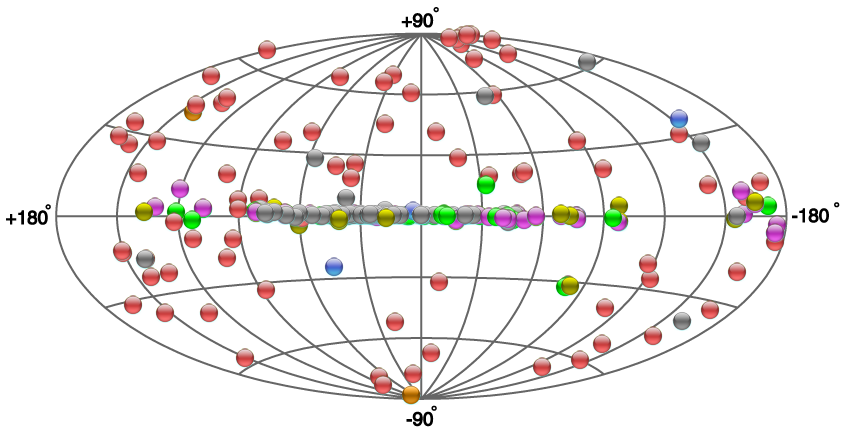
\includegraphics[width=\textwidth]{Images/tevcat.png}
\caption{Zu sehen sind alle von TeVCat registrierten und kategorisierten VHE-Quellen (ab einer Energie von $E~>50\unit{GeV}$\cite{TeVCat2}). Die roten Punkte stehen beispielsweise für AGNs, die Violetten für PWNs und die Grauen für unbekannte und unidentifizierte Quellen. \cite{TevCat}}
\label{img:tevcat}
\end{figure}


\section{Detektion von Strahlung}
Prinzipiell lässt sich zwischen bodengestützter und satellitengestützter $\gamma$-Astronomie unterscheiden. Durch den Einsatz von Satelliten vermeidet man den störenden Einfluss der Erdatmosphäre, muss dafür allerdings Abstriche in der Größe der Detektoren machen und mit hohen Kosten kalkulieren. Hier soll sich nur mit der bodengestützten Variante beschäftigt werden, die günstiger ist und nicht in der Größe beschränkt ist. Dazu verwendet man sogenannte IACTs (Imaging Atmospheric Cherenkov Telescopes), die die Strahlung nur indirekt detektieren.

\subsection{Luftschauer}
Die Atmosphäre ist nur für Photonen im optischen und radiowellen Bereich durchsichtig. Treten hochenergetische Photonen in die Atmosphäre ein, findet Paarbildung statt. Das entstehende Elektron bzw Positron ist ebenfalls hochenergetisch und verliert hauptsächlich durch Bremstrahlung Energie, worauf die entstehenden Photonen wieder durch Paarbildung wechselwirken können. Die Strahlungslängen für Paarbildung und Bremsstrahlung sind ungefähr gleich lang, sodass die Anzahl der Teilchen mit absteigender Höhe exponentiell zunimmt, wohingegend die durchschnittliche Energie der Teilchen exponentiell abnimmt. Der Luftschauer endet in einer Höhe von ungefähr 10km 
\cite{iwas}, wenn die Teichen niederenergetisch sind und die restliche Energie über Ionisation verlieren.
\begin{equation}
E_n=\frac{E_0}{2^n}
\end{equation}\\
Neben den oben beschriebenen elektromagnetischen Schauern existieren noch hadronische und myonische Schauer. Hadronische Schauer entstehen wenn hochenergetische Hadronen in die Atmosphaere eindringen. Durch die Wechselwirkung von Hadronen entstehen häufig neutrale Pionen, die wiederum in Photonen zerfallen, wodurch wiederum ein elekromagnetischer Schauer entsteht, der allderdings einen anderen Ursprung hat. %Entstehen Myonen in einem Schauer, so besteht das Problem, dass diese kaum Energie abgeben und bei hoher Geschwindigkeit den Erdboden erreichen. Somit gibt nur ein Teil des Schauers die Energie ab und die Messung weicht von der Realität ab.

\subsection{Tscherenkow-Strahlung}
Tscherenkow-Strahlung tritt auf, wenn sich geladene Teilchen in Materie schneller als die Lichtgeschwindigkeit in diesem Medium bewegen. Hierbei polarisiert das geladene Teilchen auf seiner Trajektorie die einzelnen Atome, die Licht sphärisch abstrahlen. Wäre das Teilchen langsamer als die Ausbreitungsgeschwindigkeit in diesem Medium, würden die Wellen destruktiv interferieren und man würde keine makroskopischen Effekte beobachten. Da sich das Teilchen allerdings schneller als das Licht bewegt, entsteht ein Kegel konstruktiver Interferenz, und ein Lichtblitz breitet sich kegelförmig mit dem Öffnungswinkel
\begin{equation}
\theta = \arccos\left(\frac{1}{\beta n}\right) \label{eq:cherenkow}
\end{equation}\\
aus, wie in Abb \ref{img:cherenkow} gezeigt. Für Luft (in Bodennähe) ergibt sich somit ein maximaler Öffnungswinkel von. Da allerdings die Dichte der Luft in der relevanten Höhe kleiner ist, ist auch der Brechungsindex näher an 1 und der Tscherenkow-Winkel beträgt noch ungefähr $\theta = 1^{\circ}$\cite{Grupen}
\begin{figure}[htbp]
\centering
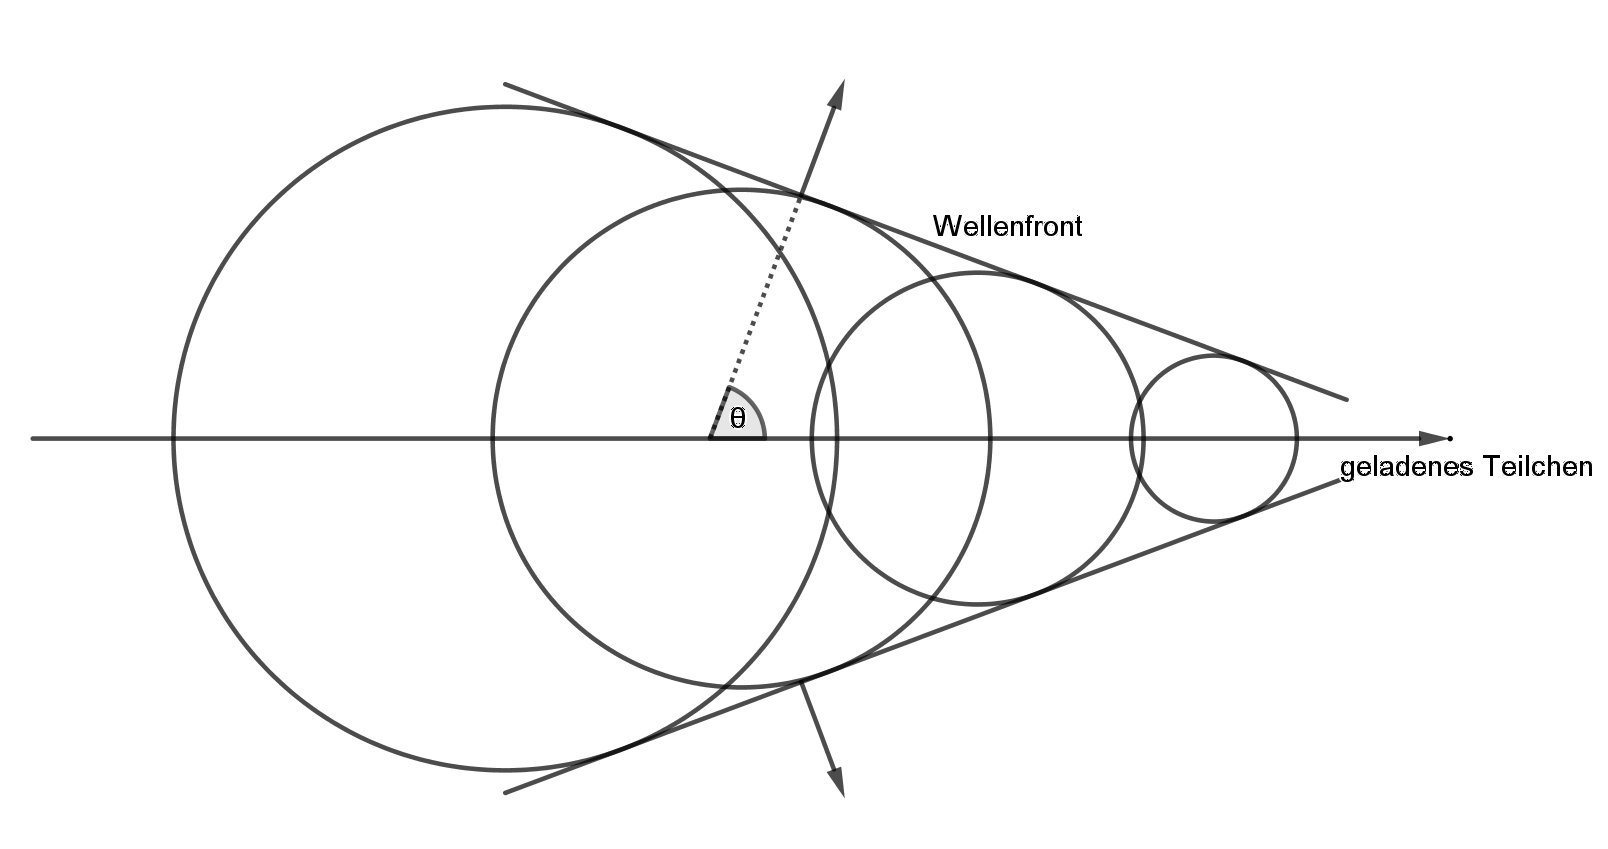
\includegraphics[width=0.7\textwidth]{Images/cherenkow.png}
\caption{Der Tscherenkow-Effekt: Ein geladenes Teilchen durchfliegt ein dielektrisches Medium mit einer Geschwindigkeit über der der Lichtgeschwindigkeit im Medium und erzeugt Wellenfronten.}
\label{img:cherenkow}
\end{figure}
Aus dem Winkel lässt sich die Geschwindigkeit des Teilchens rekonstruieren und bei bekannter Masse des Teilchens (in elektromagnetischen Schauern entstehen Elektronen als geladene Teilchen) auch der Impuls und die Energie.

\subsection{Bodengestützte Detektion der Tscherenkow-Strahlung}
Ziel der bodengestützten Variante ist es, das Tscherenkow-Licht der sekundären Teilchen aus dem elektromagnetischen Schauer zu detektieren. Bei einem Tschernekow-Winkel von $\theta=1^{\circ}$ in $10\unit{km}$ Höhe und senkrechter Einstrahlung ergibt sich ein Lichtpool am Boden mit einem Durchmesser von $250\unit{m}$ \cite{DesignConcept}. Somit müssen effektive Flächen in der Größenordnung von $10^4$ bis $10^5\unit{m^2}$ abgedeckt werden um den gesamten Schauer zu detektieren. Typischerweise entstehen bei einem VHE-Photon $10^8-10^9$ Photonen, die innerhalb von wenigen Nanosekunden abgegeben werden. Am Boden hat man somit typische Intensitäten von $10^3\unit{\frac{1}{m^2}}$ die detektiert werden müssen.
Dazu verwendet man IACTs, die aus einem Reflektor und einem Detektor bestehen. Der Reflektor besteht aus einem oder häufig aus mehreren Spiegeln, die das Tscherenkow-Licht in der Brennebene bündeln. Bei großen Teleskopen muss der Reflektor parabolisch sein und bei kleineren wird darauf häufig aus Kostengründen verzichtet, da jeder einzelne Spiegel eine individuelle Brennweite braucht.
Als Detektor wird eine Tscherenkow-Kamera verwendet, die eine typische Auflösung von 2000 Pixeln und Zeitauflösung $10\unit{ns}$\cite{CherenkovCam} hat. Das die Auflösung im Vergleich zu CCD Kameras eher gering ist, liegt daran, dass der Detektor sehr wenige Photonen in einer sehr kurzen Zeit detektiert werden müssen. Dazu verwendet man Photomultiplier.
Aus den aufgenommenen Daten lässt sich mit Hilfe von Monte-Carlo-Simulationen die Richtung und die Energie des detektierten Photons rekonstruieren. 

\begin{figure}[htbp]
\centering
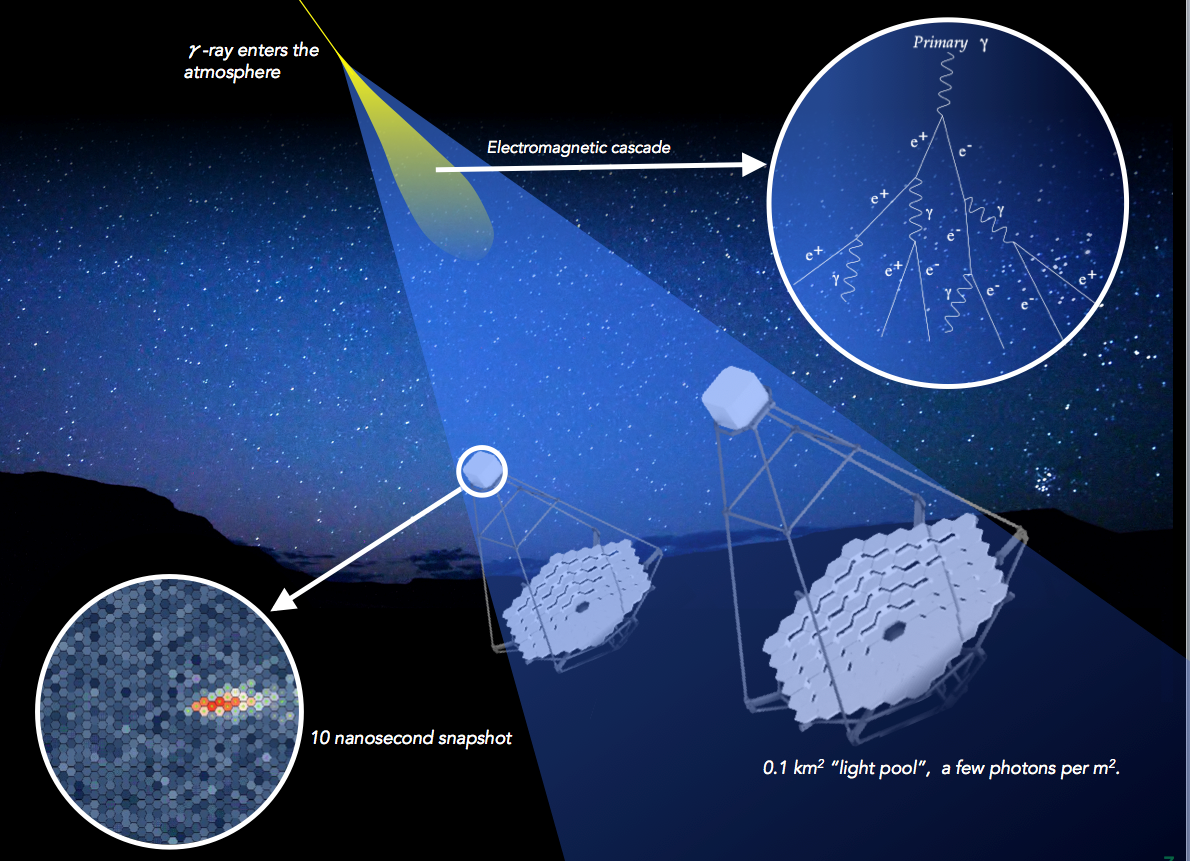
\includegraphics[width=\textwidth]{Images/detection.png}
\caption{Detektion hochenergetischer Strahlung: Das in die Atmosphäre eintretende Photon erzeugt einen elektromagnetischen Luftschauer (oben rechts) der wiederum Cherenkovlicht erzeugt, welches am Boden mit IACTs detektiert werden kann. Ein Detektionsbild ist unten links zu sehen.}
\label{img:detection}
\end{figure}

\chapter{Das Cherenkov Telescope Array}
Mit dem Bau des Cherenkov Telescope Arrays (CTA) werden verschiedene Ziele verfolgt \cite{NextGen}:
\begin{itemize}

\item Abdeckung des Energiebereichs von 30GeV bis 100TeV
\item Verbesserung der Sensitivitaet um eine Groessenordnung im Vergleich zur aktuellen Generation (H.E.S.S., VERITAS und MAGIC)
\item Verbesserung der Winkelaufloesung auf $0,1^{\circ}$ bei 0,1TeV und $0,05^{\circ}$ bei 1TeV
\item Verbesserung der Energieaufloesung auf 25\% bei 50GeV und 10\% bei 1TeV
\item Entdeckung einer grossen Anzahl von Quellen bekannter Klassen
\item Entdeckung neuer Quellen (zum Beispiel Quellen GRBs)
\item Abdeckung des gesamten Himmels (nord+sued)
\end{itemize}

\section{Design-Konzept}
Um sowohl die suedliche als auch die noerdliche Hemnisphaere abzudecken, wird das CTA in der Atacamawueste in Chile und auf der zu Spanien gehoerenden Insel La Palma errichtet.
\subsection{Teleskoptypen}
Fuer das CTA werden drei Teleskope unterschiedlicher Groesse entwickelt
\begin{description}
\item[Small Sized Telescope (SMT)]\hfill \\
Das kleinste Teleskop ist sensitiv im Bereich von 1TeV bis 300TeV und wird eingesetzt um Schauer grosser Energie zu detektieren. Momentan werden drei verschiedene Varianten entwickelt, die zu einem harmonisiert werden sollen. Das SST 1M ist eine kleinere Variante des MST und SST-2M  ASTRI und das SST-2M GCT basieren auf dem Prinzip eines Schwarzschild-Couder Designs. Das SST soll einen Reflektordurchmesser von ca. 4m haben.
\item[Medium Sized Telescope (MST)]\hfill \\ 
Das MST basiert auf einem modifiziertem Davies-Cotton-Design und hat einen Durchmesser von 12m. Mit einem Sensitivitaetsbereich von 150GeV bis 5TeV deckt es den Kernbereich des CTAs ab.
\item[Large Sized Telescope (LST)]\hfill \\
Die groessten Teleskope des CTA werden einen Reflektordurchmesser von 23m um auch Strahlung niedriger Energie zu detektieren. Da aufgrund der Groesse eine Bauweise aus Stahl zu schwer waere, werden diese Teleskope aus kohlefaserverstaerktem Kunststoff gebaut. Das hat zum Vorteil, dass die Teleskope zwar leichter werden, aber es hat auch den Nachteil, dass die Bauteile durch Bewegung des Teleskops staerker verbiegen, was das Pointing erschwert. Aufgrund der Groesse dieser Teleskope reicht es nicht mehr die Reflektoren dieser Teleskope sphaerisch zu bauen, sondern parabolisch. Hierbei steigt der Aufwand, da jeder einzelne Spiegel eine individuelle Brennweite hat.
\end{description}
\begin{figure}[htbp]
\centering
\includegraphics[width=\textwidth]{Images/TelescopeTypes.jpg}
\caption{Die drei verschieden grossen Teleskope des CTA: links die drei Varianten des SMT, in der Mitte das MST und rechts das LST}
\label{img:TelescopeTypes}
\end{figure}

\subsection{Arrays}
Um den gesamten Himmel abdecken zu koennen wird jeweils eine Anlage auf der Nordhalbkugel un der Suedhalbkugel errichtet.
\begin{description}
\item[suedliche Hemnisphaere]\hfill \\
Die groessere der beiden Anlagen wird in der Atacamawueste in Chile errichtet und besteht aus allen drei Teleskoptypen, die auf einer Flaeche von $4km^2$ verteilt sind \ref{img:ArrayLayout}, um so den gesamten Energiebereich des CTAs abzudecken
\item[noerdliche Hemnisphaere]\hfill \\ 
Auf der spanischen Insel La Palma wird die noerdliche Anlage errichtet. Hier steht eine kleinere Flaeche zur Verfuegung und es wird auf die kleinen Teleskope verzichtet, wodurch der Energiebereich auf 20GeV bis 20TeV begrenzt ist.
\end{description}

\begin{figure}[htbp]
\centering
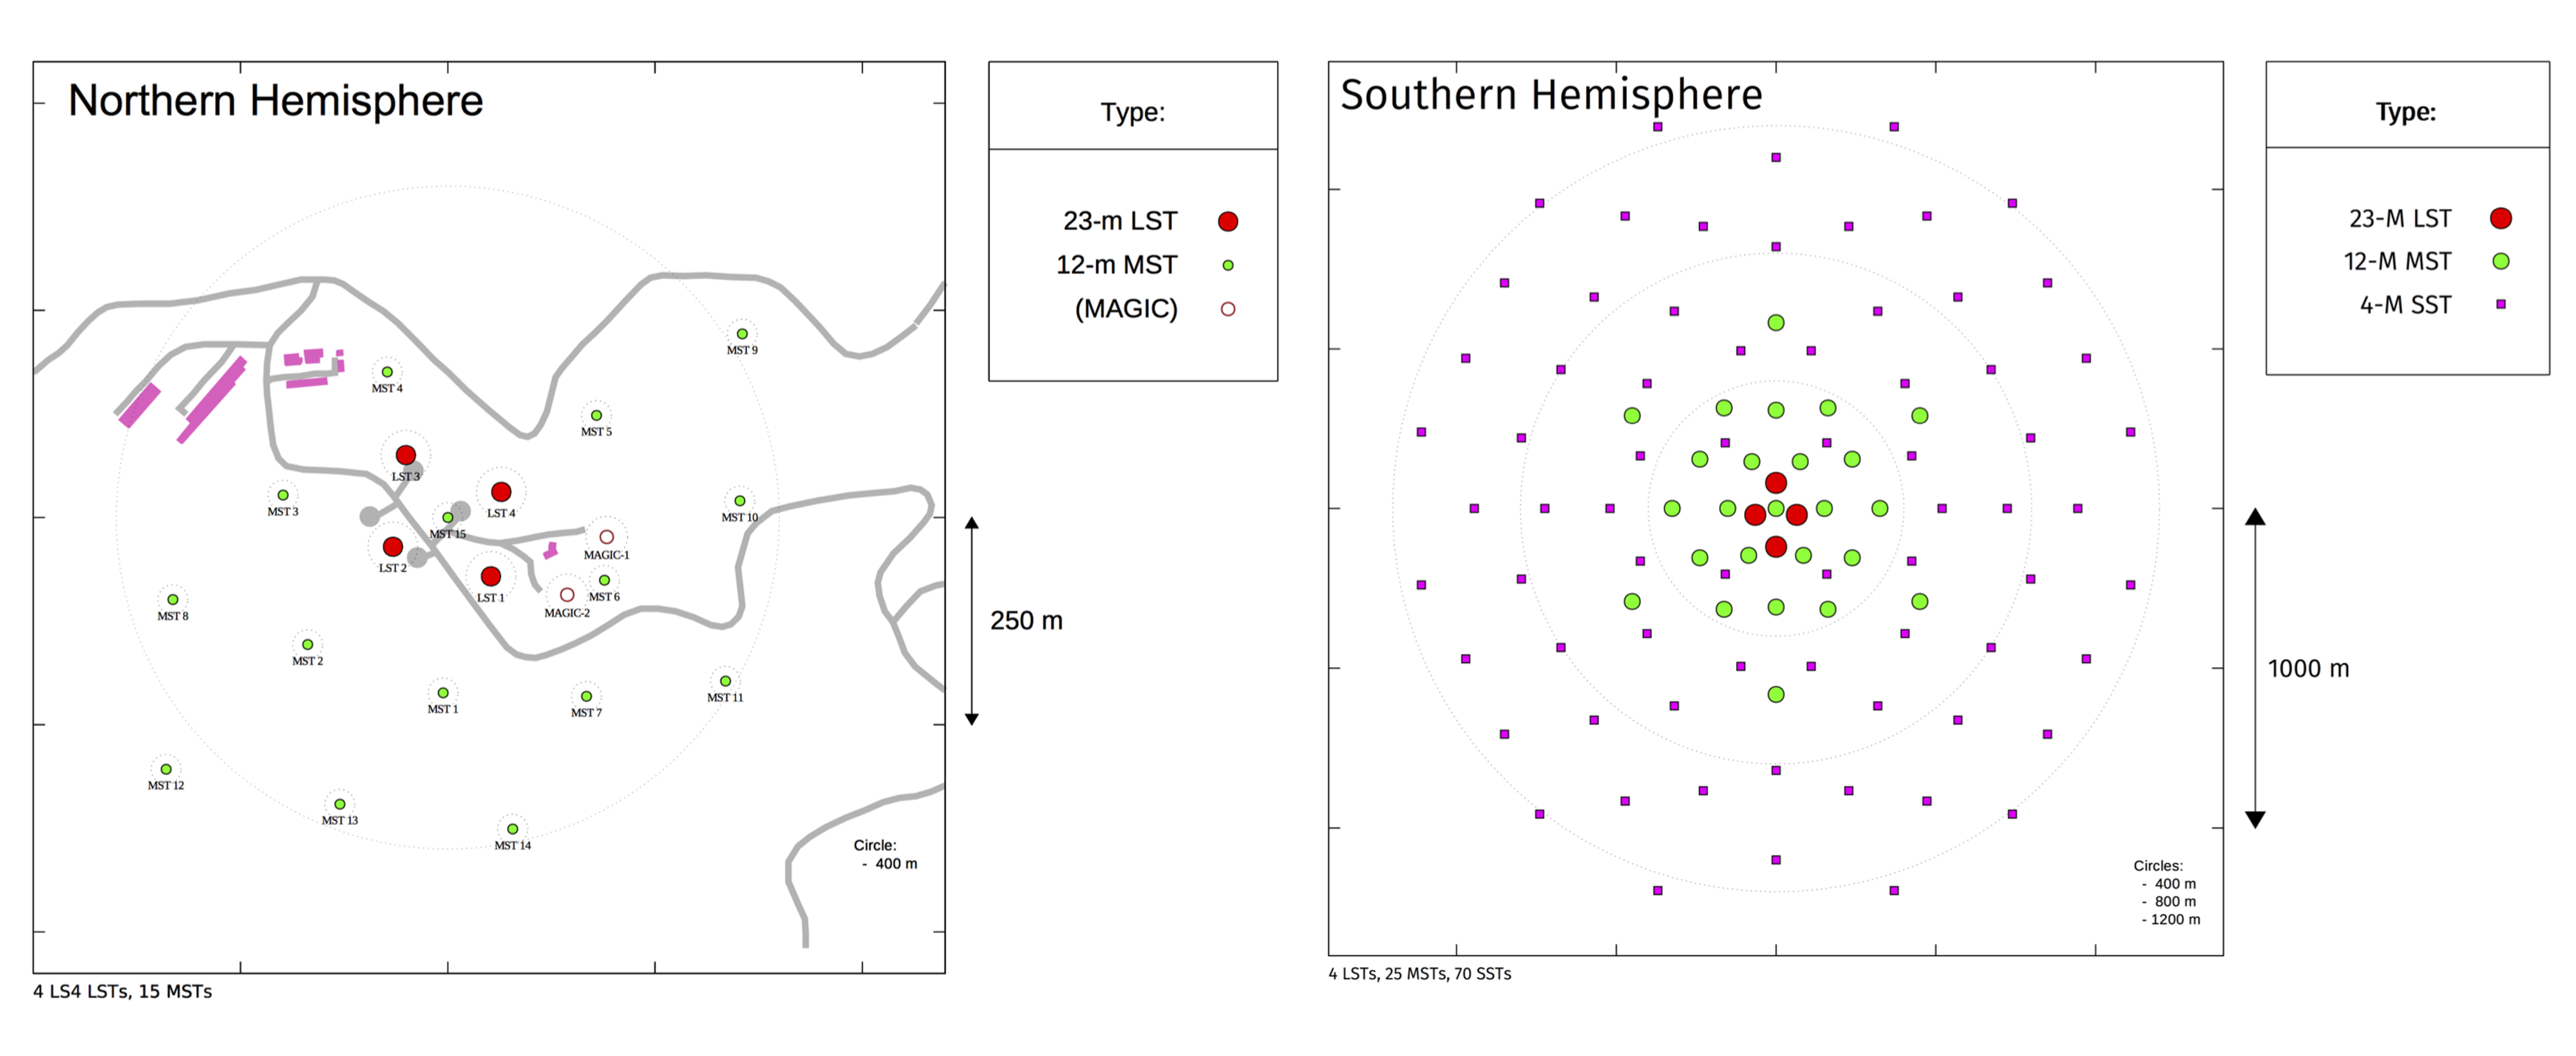
\includegraphics[width=\textwidth]{Images/ArrayLayout.png}
\caption{Der geplante Aufbau der Arrays auf La Palma und in der Atacamawueste: Auf La Palma werden zunaechst nur die beiden groesseren Teleskoptypen am Krater des Vulkans errichtet. In der Atacamawueste werden alle drei Teleskoptypten verwendet. Aufgrund der grossen freien Flaeche kann hier auch ein grosser Bereich symmetrisch abgedeckt werden.}
\label{img:ArrayLayout}
\end{figure}

\section{Prototyp in Adlershof}
In Adlershof wurde 2012 vom DESY ein Prototyp des MSTs errichtet um den mechanischen Aufbau zu testen, Pointingmodelle zu entwickeln und um die einzelnen Spiegel zu testen und auszurichten.

\subsection{Kameras des MST}
Der Prototyp des MST besitzt drei Kameras in der Mitte des Reflektors. Die Sky-CCD, für die im hier folgenden ein Pointingmodell entwickelt wird, ist schräg montiert, sodass sie am Detektorarm vorbei guckt um Bilder des Nachthimmels aufzunehmen. Aus diesen Bildern lassen sich mithilfe der Astrometry-Software die Koordinaten der Kamera bestimmen, die als die wahren Koordinaten angenommen werden.

\subsection{Koordinatens des MST}
Das MST benutzt ein Koordinatensystem aus zwei Winkeln und aehnelt den Kugelkoordinaten. Der Azimutwinkel ($az$) beschreibt die Auslenkung in der Ebenenen und lauft von $-180^{\circ}$ bis $180^{\circ}$, wobei es fuer $az=0^{\circ}$ in Richtung Norden ausgerichtet ist. Der Elevationswinkel $el$ lauft von $0^{\circ}$ bis $90^{\circ}$ wobei $el=90^{\circ}$ dem Zenit entspricht. Da es bei der Entwicklung von Pointingmodellen von Vorteil sein kann, wenn man in kartesischen Koordinaten rechnet, wurde hier die Konvention verwendet, dass Nordrichtung der x-Richtung, die Westrichtung der y-Richtung und die Zenitrichtung der z-Richtung entspricht.
\begin{figure}[htbp]
\centering
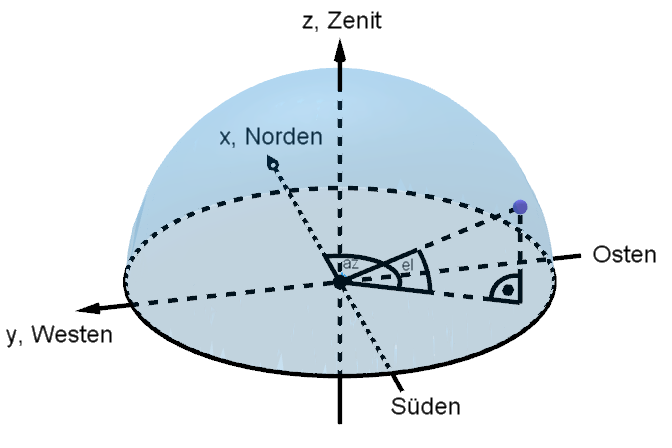
\includegraphics[width=0.7\textwidth]{Images/coordinates.png}
\caption{Die verwendeten Koordinaten}
\label{img:coordinates}
\end{figure}
\subsection{Bestimmung der Bildkoordinaten durch astronometry.net}
Aus den mit der Kamera aufgenommen Bildern lassen sich mithilfe der astronometry.net Software die einzelnen Koordinaten der Bilder und die Groesse des Bildausschnitts bestimmen. Auf den einzelnen Bildern werden Sterne erkannt, die jeweils zu Tripplets zusammengeschlossen werden. Diese Tripletts werden mit zwei Sternenkatalogen 
\begin{itemize}
\item USNO-B: Ein Katalog mit ungefaehr einer Milliarde OBjekten (Sterne und Galaxien)
\item TYYCHO-2 Ein Katalog mit den 2.5 Millionen hellsten Sternen
\end{itemize}
Die Software kommt auch mit Fehlern wie fehlenden und zu vielen Objekten klar.

%\chapter{Bildanalyse}
Zu Beginn war der MST Protoyp in Adlershof noch nicht mit einem Cherenkovdetektor ausgestattet, sondern nur mit einfachen CCDs. Mit diesen wurde die Helligkeit des Nachthimmels beobachtet.

\section{CCD Kameras}

\section{Verwendete Kamera}
Das MST ist mit verschiedenen Kameras ausgestattet, wobei nur Bilder der sogenannten Sky-CCD verwendet wurden. Die Sky-CCD ist eine ist eine Kamera des Typs Prosilica GC 1350 mit folgenden technischen Daten.

Die Bilder wurden mit mit drei verschieden Belichtungszeiten (1s, 10s und 20s) und vier verschieden gain-Verstärkungsstufen (0dB, 7dB,14dB und 21dB) aufgenommen. Die Bilder wurden in Schwarz-Weiß mit einer Farbtiefe von 8Bit aufgenommen, das heißt jedem Pixel wird ein Wert von 0 bis 255 zugewiesen, wobei der Wert 255 der maximalen Helligkeit entspricht.

\section{Helligkeit der Bilder}
Um die Helligkeit der Bilder zu bestimmen wurde auf das arithmetische Mittel verzichtet, da dieses durch den Einfluss heißer Pixel in Richtung zu hoher Helligkeit verschoben wird. Heiße Pixel sind Pixel, die nicht ordnungsgemäß funktionieren und nicht proportional auf das einfallende Licht reagieren, sondern schneller hell werden. Gerade bei längeren Belichtungszeiten kommt es so vor, dass diese Pixel auch bei eher dunklen Bildern des Nachthimmels den maximalen Helligkeitswert annehmen. Um diesen Effekt zu minimieren, wurde jeweils der Median der Verteilung berechnet. Da die Helligkeit der Pixel der Digitalkamera nur ganzzahlige Werte annehmen kann, aber gerade im dunklen Bereich eine präzisere Helligkeit erreicht werden soll, wurde die Verteilung innerhalb eines Bins als kontinuierlich. Zudem wurde noch die Breite der Verteilung berechnet. Dazu wurde der Bereich einer Standardabweichung also 37, \% links und rechts des zuvor berechneten Medians gewählt.

Zur Analyse des Zusammenhangs der Belichtungszeit bzw des gains auf die Helligkeit der Bilder wurde der Datensatz "run 199" verwendet, der am von bis aufgenommen wurde. Für jedes einzelne Bild wurde die Belichtungszeit und der gain sowie wie oben beschrieben der Median der Helligkeitsverteilung sowie deren Breite bestimmt

\section{Korrelation der Werte}
Im folgenden soll untersucht werden, wie sich Helligkeit und Breite in Abhängigkeit der Belichtungszeit und des gains verhalten.

\subsection{Abhängigkeit von der Belichtungszeit}
Eine längere Belichtungszeit bedeutet, dass die Blende der Kamera länger geöffnet bleibt. Daraus folgt die Erwartung, dass die Anzahl der detektierten Photonen proportional steigt und somit auch der Median der Helligkeitsverteilungen.

\subsection{Abhängigkeit vom gain}

\section{Fazit}
\chapter{Pointingmodell}
Das Pointing von Teleskopen beschäftigt sich damit, dass das Teleskop so ausgerichtet wird, wie es erwünscht ist. Häufig ist das Problem, dass die eingestellte Position nicht exakt mit der gewünschten Position übereinstimmt. Gründe dafür können Fehler in der Präzision oder auch die Elastizität einzelner Bauteile sein. Da man die aufgenommen Daten mit den Bekannten Postionen am Himmel vergleichen kann, kann man versuchen ein Modell zu finden, welches die Fehler verkleinert oder im Idealfall sogar eliminiert.

\section{Koordinatens des MST}
Als geeignetes Koordinatensystem für den Betrieb eines Teleskops erweist sich ein mit zwei Winkeln zu beschreibendes System, das den Kugelkoordinaten ähnelt. Der Azemutwinkel behält seinen Namen und zeigt in der Regel bei $0^\circ$ in Richtung Norden. Der Polarwinkel behält ebenfalls seine Bedeutung und wird Elevation genannt.

\section{Kameras des MST}
Der Prototyp des MST besitzt drei Kameras in der Mitte des Reflektors. Die Sky-CCD, für die im hier folgenden ein Pointingmodell entwickelt wird, ist schräg montiert, sodass sie am Detektorarm vorbei guckt um Bilder des Nachthimmels aufzunehmen. Aus diesen Bildern lassen sich mithilfe der Astrometry-Software die Koordinaten der Kamera bestimmen, die als die wahren Koordinaten angenommen werden.

\section{Entwicklung von Pointingmodellen}
Da man aus den gewünschten Koordinaten der CCD die Koordinaten des Drives bestimmen lässt, drückt man sie als Funktion voneinander aus.
\begin{equation}
az_D=f_{az}(az_C,el_C)
el_D=f_{el}(az_C,el_C)
\label{eq:pointingprinciple}
\end{equation}\\

Diese Funktionen werden so optimiert, dass die Gleichung möglichst gut erfüllt wird.

\section{Vereinfachtes Pointingmodell f\"ur feste Azimutwerte}
Zunächst wurde ein Datensatz (run281), bei dem die vier feste Elevationswerte am Drive eingestellt wurden, verwendet. In diesem Modell wird die Position der Kamera durch zwei Drehungen beschrieben (eine um die x-Achse und eine um die z-Achse). Somit lässt sich die Position des Drives bzw der Kamera durch die Richtungsvektoren beschreiben.
%Vektoren in Gleichung
Da sich diese Vektoren durch Transformationen die unabhängig von el und az sind ineinander überführen lassen, kann das Modell auch entwickelt werden, indem die Drive und CCD Koordinaten in \ref{eq:pointingprinciple} untereinander tauscht. Das hat zum Vorteil, dass man die Funktionen nur für eine Variable fitten muss.\\
Die Richtungsvektoren lassen sich durch zwei weitere Drehungen um den Elevationswinkel und den Azimutwinkel in Position bringen. Aus den resultierenden Vektoren lassen sich wiederum die wahren Azimut- und Elevationswerte bestimmen.
\begin{equation}
az=\arctan\left(\frac{y}{x}\right)
el=\arcsin(z)
\end{equation}\\
wobei $x$,$y$ und $z$ den einzelnen Koordinaten der Vektoren entsprechen. Somit ergeben sich für dieses Modell folgende Funktionen.
%Pointingfunktionen
Hier müssen noch die beiden Winkel durch Fits am Datensatz bestimmt werden. Die Fits wurden jeweils für die vier Azimutwerte und die beiden Pointingfunktionen unabhängig durchgeführt, sodass sich für jeden Fit neue Parameter ergeben. Zusätzlich wurden konstante Fehlerbalken berechnet, die die Bedingung $\frac{\chi^2}{doF}$ erfüllen. Diese ergeben sich durch.
\chapter{Anwendung des Pointingmodells auf Daten des Teleskops}
\label{ch:auswertung}
Um das in Kapitel \ref{ch:pointing} entwickelte Pointingmodell zu testen, wurde mit dem Prototyp des MST ein Datensatz aufgenommen um
\section{Datensatz}
Der verwendete Datensatz wurde am MST-Prototyp in Adlershof in der Nacht vom 4. auf den 5. Juli 2018 im Zeitraum von 21:00 UTC bis 1:45 UTC aufgenommen. Dazu wurden 105 Postionen beobachtet wobei das Teleskop anfangs Richtung Zenit stand und sich dann in einer abwärtslaufenden Spirale befand. An jeder Position wurden 4 Bilder aufgezeichnet, wovon zwei eine Belichtungszeit von 20 Sekunden hatten. Die jeweils zweiten Bilder mit dieser Belichtungszeit aufgenommenen Bilder wurden verwendet um mithilfe einer Software die Koordinaten des Bildmittelpunktes zu bestimmen. Das war bei 100 Bildern erflolgreich.
\begin{figure}[htbp]
\centering
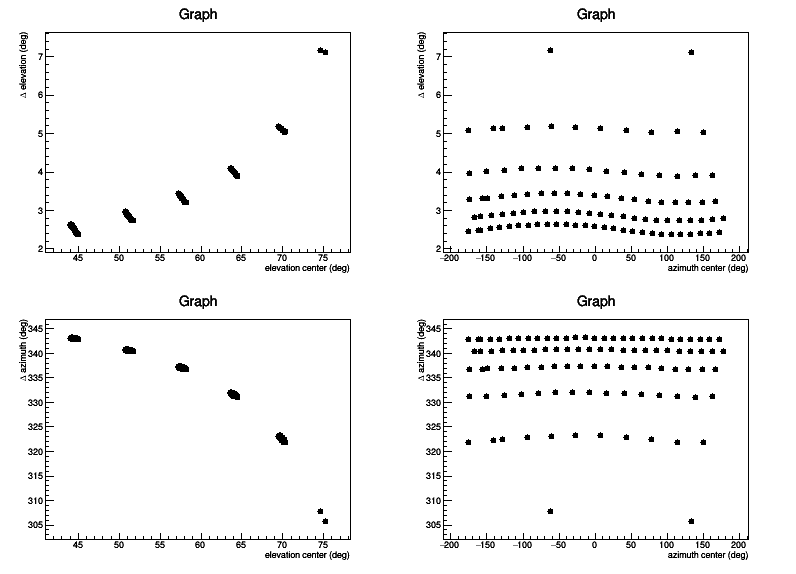
\includegraphics[width=\textwidth]{../341/data2.png}
\label{img:dataset}
\caption{Zu sehen sind die Abweichungen zwischen gemessenen und eingestellten Koordinaten in Abhängigkeit der gemessenen Koordinaten}
\end{figure}
Der zur Analyse verwendete Datensatz besteht somit aus 100 Einträgen, die jeweils die Elevations und Azimutkoordinaten des Drivesystems (also der am Teleskop eingestellten Koordinaten) und der tatsächlichen (also der Koordinaten des Bildmittelpunktes).
\section{Programm}
Um das Pointingmodell auf Konsistenz zu überprüfen wurde ein Programm in ROOT geschrieben, welches die Differenzen der vom Pointingmodell (Index P) bestimmten Werte mit den gemessenen (Index M) Werten berechnet und analysiert. Da die oben entwickelten Pointingmodelle noch freie Parameter haben, die vom Teleskop abhängen werden diese durch eine Regression der Daten bestimmt. Da das Pointingmodell aus zwei Funktionen besteht (jeweils eine für die Elevation und den Azimut), die jedoch von den gleichen Parametern abhängen, muss hier ein kombinierter Fit durchgeführt werden. Dazu wird eine Hilfsvariable eingeführt, die die Summe der Quadrate der Differenzen von Messwerten und vorhergesagten Werten für feste Werte der freien Parameter bestimmt.
\begin{equation}
Q=\sum^N_{i=1}\left(P_i-M_i\right)^2
\end{equation}
Durch die Bildung der Quadrate können sich Abweichungen nach oben und unten nicht gegenseitig kompensieren und die Hilfsvariable ist somit ein Maß für die Abweichung von Modell mit den gewählten Parametern und Messwerten. Die besten Parameter erhält man, indem man die Variable minimiert. Dazu wurde die in ROOT integrierte Funktion TMinuit verwendet, die zudem noch die Standardabweichung der Parameter ausgibt. Um die Güte des Modells bestimmen zu können wird noch die Größe $\frac{\chi^2}{doF}$ verwendet um die Fehler der Messwerte zu bestimmen, in denen das Modell mit dem Datensatz übereinstimmt. Die Größe $\frac{\chi^2}{doF}$ ist definiert als
\begin{equation}
\frac{\chi^2}{doF}=\sum^N_{i=1}\frac{\left(P_i-M_i\right)^2}{\sigma_i^2}
\end{equation}
wobei hier $\sigma_i$ der Fehler des Wertes i ist und $doF$ der Anzahl der Freiheitsgraden entspricht. Diese berechnet sich durch
\begin{equation}
doF=N-\textrm{Anzahl der Parameter}
\end{equation}
Der perfekte Wert für $\frac{\chi^2}{doF}$ ist 1. Unter der Anahme, dass die Fehler $\sigma$ alle gleich groß sind, lassen sich diese wie folgt berechnen
\begin{equation}
\sigma=\sqrt{\frac{\sum^N_{i=1}\left(P_i-M_i\right)^2}{doF}}=\sqrt{\frac{Q}{doF}}
\end{equation}
Interessant ist es auch, sich die Korrelation der Parameter untereinander anzugucken. Die Korrelation beschreibt die Beziehung der zwischen einzelnen Parametern. Hier wird dazu der Korrelationskoeffizient nach Pearson verwendet, der ausschließlich die lineare Korrelation berücksichtigt. Um diesen zu berechnen wird zunächst die Korelationsmatrix
\begin{equation}
COV(X,Y)=\left<\left(X-\left<X\right>\right)\cdot\left(Y-\left<Y\right>\right)\right>
\end{equation}
berechnet. Auf der Hauptdiagonale stehen die Varianzen, aus denen sich die Fehler der Parameter bestimmen lassen:
\begin{equation}
\sigma_X=\sqrt{COV(X,X)}=\sqrt{VAR(X)}
\end{equation}
Der Korrelationskoeffizient lässt sich nun durch
\begin{equation}
\rho_{XY}=\frac{COV(X,Y)}{\sigma_X\sigma_Y}
\end{equation}\\
Um die Qualität der jeweiligen Pointingmodelle beurteilen zu können, werden jeweils vier Plots ausgegeben, die die jeweiligen Differenzen der bestimmten und gemessenen Koordinaten angeben
\begin{equation}
f=el_M-el_P \quad \textrm{bzw} \quad f=az_M-az_P
\end{equation}
\section{Anwendung auf das Pointingmodell mit 2 Parametern}
Zunächst wird das Modell mit den Parametern $el0$ und $az0$ untersucht.
\subsection{Abhängigkeit der Drivekoordinaten in Abhängigkeit der CCD-Koordinaten}
Um die Koordinaten des Teleskops anhand der Koordinaten der CCD-Kamera vorherzusagen wird das aus den Gleichungen \ref{eq:elC2D} und \ref{eq:azC2D} verwendet. Berechnet man die Parameter mit dem oben beschriebenen Programm so erhält man die Parameter in Tabelle \ref{tab:C2D}. Die Abweichungen zwischen Vorhersage und gemessenen Werten sind in Abbildung \ref{img:C2D} zu sehen.
\begin{figure}[htbp]
\centering
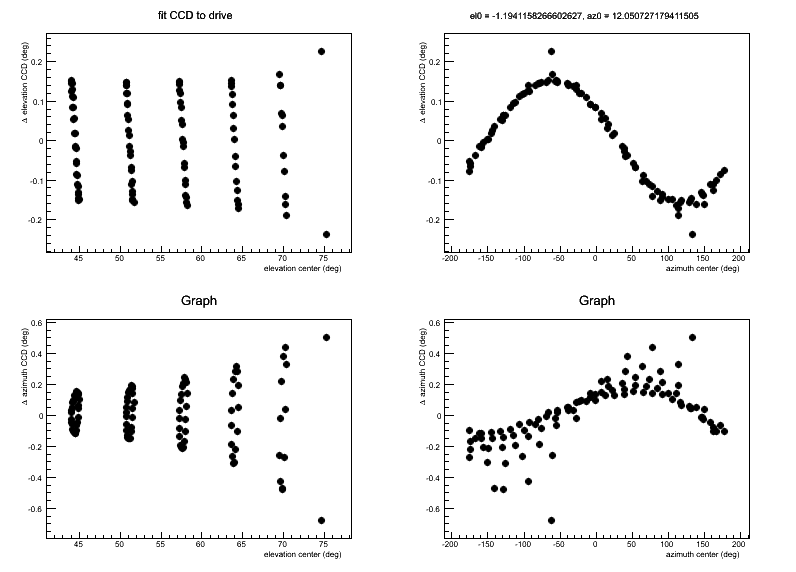
\includegraphics[width=\textwidth]{../341/run341C2D.png}
\caption{Die Drivekoordinaten in Abhängigkeit der CCD-Koordinaten}
\label{img:C2D}
\end{figure}

\begin{table}[htbp]
\centering
\begin{tabular}{rcl}
\toprule
$el0$ &=& $(-1,1941\pm0,0098)^{\circ}$\\
$az0$ &=& $(12,0507\pm0,0019)^{\circ}$\\
$\sigma$ &=& $0,23^{\circ}$\\
$\rho_{el_0,az0}$ &=& $0,1576$\\
\bottomrule
\end{tabular}
\label{tab:C2D}
\caption{Die für das Pointingmodell mit 2 Parametern bestimmten Werte}
\end{table}

\subsection{Abhängigkeit der CCD-Koordinaten in Abhängigkeit der Drivekoordinaten}
Für das inverse Modell werden die Gleichungen \ref{eq:elD2C} und \ref{eq:azD2C} verwendet. Mit diesen kommt man auf die Werte in Tabelle \ref{tab:D2C} und die in Abbildung \ref{img:D2C} gezeigten Abbildungen.
\begin{figure}[htbp]
\centering
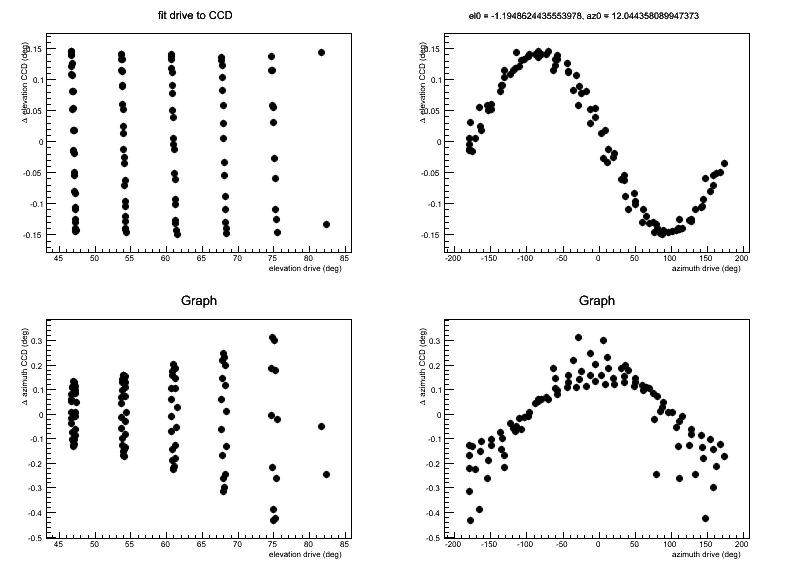
\includegraphics[width=\textwidth]{../341/run341D2C.png}
\caption{Die CCD-Koordinaten in Abhängigkeit der Driveoordinaten im Zwei-Parameter-Modell}
\label{img:D2C}
\end{figure}

\end{figure}
\begin{table}[htbp]
\centering
\begin{tabular}{rcl}
\toprule
$el0$ &=& $(-1,184\pm0,008)^{\circ}$\\
$az0$ &=& $(12,048\pm0,004)^{\circ}$\\
$\sigma$ &=& $0,19^{\circ}$\\
$\rho_{el_0,az0}$ &=& $-0,4698$\\
\bottomrule
\end{tabular}
\label{tab:D2C}
\caption{Die Drive-Koordinaten in Abhängigkeit der CCD-Koordinaten im Zwei-Parameter-Modell}
\end{table}

\section{Anwendung auf das Pointingmodell mit 4 Parametern}
Im folgenden wird das obige Modell auf vier Parameter erweitert indem wie in Abschnitt \ref{se:4par} beschrieben jeweils ein konstanter Wert zu den Drive-Koordinaten hinzuaddiert wird.
\subsection{Abhängigkeit der Drivekoordinaten in Abhängigkeit der CCD-Koordinaten}
Werden die Formeln \ref{eq:elC2D4} und \ref{eq:azC2D4} verwendet erhält man die in Abbildung \ref{img:C2D4} gezeigten Differenzen und die in Tabelle \ref{tab:C2D4} aufgelisteten Werte.
\begin{figure}[htbp]
\centering
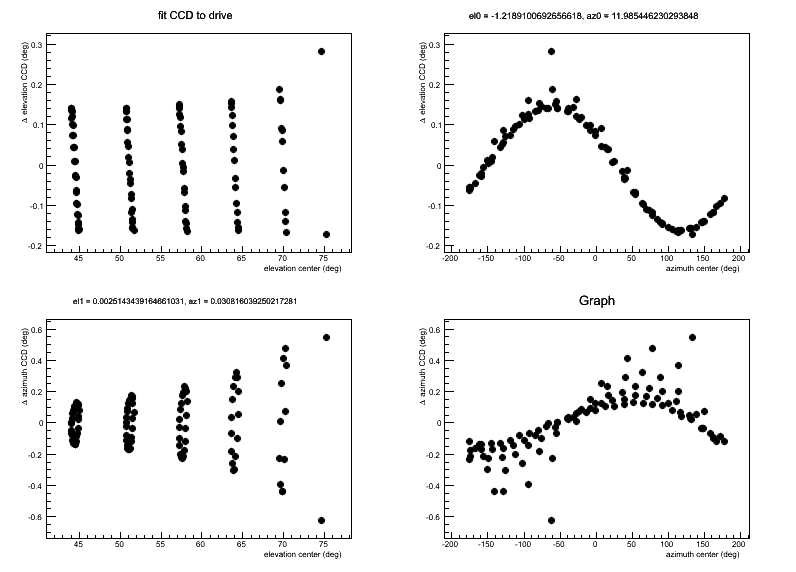
\includegraphics[width=\textwidth]{../341/run341C2D_4par.png}
\caption{Die Drivekoordinaten in Abhängigkeit der CCD-Koordinaten}
\label{img:C2D4}
\end{figure}
\begin{table}[htbp]
\centering
\begin{tabular}{rcl}
\toprule
$el0$ &=& $(-1,21891\pm 0,03924)^{\circ}$\\
$az0$ &=& $(11,9854\pm0,2072)^{\circ}$\\
$el_1$ &=& $(0,00251434\pm 0,0001839)^{\circ}$\\
$az0$ &=& $(0,03080816\pm0,2149)^{\circ}$\\
$\sigma$ &=& $0,23^{\circ}$\\
$\rho_{el_0,az_0}$ &=& $0,8691$\\
$\rho_{el_0,el_1}$ &=& $-0,8417$\\
$\rho_{az_0,az_1}$ &=& $-0,9358$\\
$\rho_{el_0,az_1}$ &=& $-0,8137$\\
$\rho_{az_0,el_1}$ &=& $-0,9709$\\
$\rho_{el_1,el_1}$ &=& $-0,8417$\\
\bottomrule
\end{tabular}
\label{tab:C2D4}
\caption{Die für das Pointingmodell mit 4 Parametern bestimmten Werte}
\end{table}

\subsection{Abhängigkeit der CCD-Koordinaten in Abhängigkeit der Drivekoordinaten}
Invertiert man das Modell, so verwendet man die Gleichungen \ref{eq:elD2C4} und \ref{eq:azD2C4}, sodass das das Programm die Werte aus Tabelle \ref{tab:D2C4} und die Abstände aus Abbildung \ref{img:D2C4} liefert.
\begin{figure}[htbp]
\centering
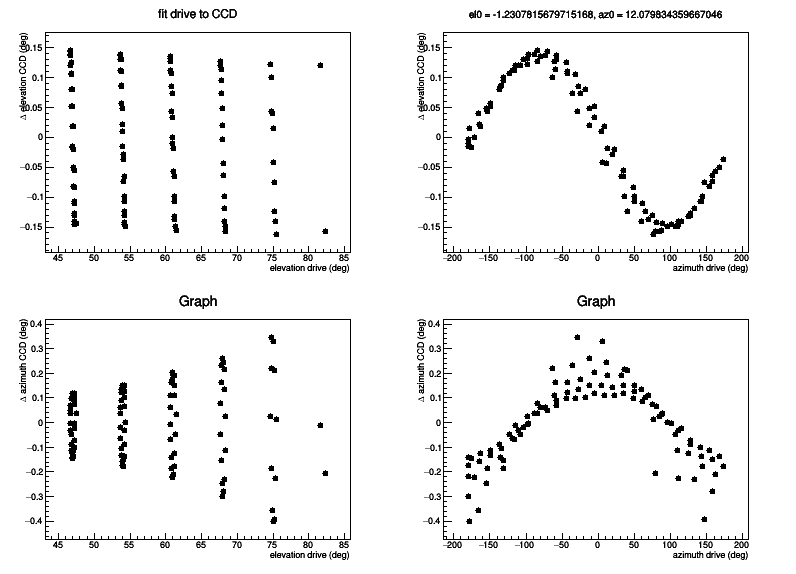
\includegraphics[width=\textwidth]{../341/run341D2C4.png}
\caption{Die CCD-Koordinaten in Abhängigkeit der Driveoordinaten}
\label{img:D2C4}
\end{figure}
\begin{table}[htbp]
\centering
\begin{tabular}{rcl}
\toprule
$el0$ &=& $(-1,19373\pm 0,9976)^{\circ}$\\
$az0$ &=& $(12,0957\pm0,04068)^{\circ}$\\
$el_1$ &=& $(0,0192352\pm 1,043)^{\circ}$\\
$az0$ &=& $(-0,0946443\pm0,1452)^{\circ}$\\
$\sigma$ &=& $0,10^{\circ}$\\
$\rho_{el_0,az_0}$ &=& $-0,009202$\\
$\rho_{el_0,el_1}$ &=& $-0,0218$\\
$\rho_{az_0,az_1}$ &=& $-0,9493$\\
$\rho_{el_0,az_1}$ &=& $-0,9954$\\
$\rho_{az_0,el_1}$ &=& $-0,03329$\\
$\rho_{el_1,el_1}$ &=& $-0,01867$\\
\bottomrule
\end{tabular}
\label{tab:D2C4}
\caption{Die für das Pointingmodell mit 4 Parametern bestimmten Werte}
\end{table}

\section{Diskussion der Korrelation}
Sieht man sich die einzelnen Korrelationen an, so erkennt man, dass sich diese für das jeweils gleiche Modell mit gleich vielen Parametern stark unterscheiden und gerade im Modell mit vier Parametern sehr starke Korrelationen auftreten.
\subsection{Unterschiedliche Korrelationen für Modelle mit gleichen Parametern}
Zunächst fällt auf, dass sich im Modell mit zwei Parametern die Korrelationskoeffizienten stark unterscheiden
\subsection{Hohe Korrelation im Modell mit vier Parametern}

\section{Systematische Abweichungen im entwickelten Pointingmodell}

\chapter{Fazit}

% usw.

%-Anhang----------------------------------------------------------

\appendix

%-Literaturverzeichnis--------------------------------------------

%\nocite{*}
%die Verwendung von bibtex ist Pflicht!!!
\bibliography{bibliography}
\bibliographystyle{plain}        %bzw. unsrtdin, alphadin, abbrvdin

%-Kapitel des Anhangs---------------------------------------------

%\chapter{\Alph{Anhang}Anhang}
\section*{Ergebnisse der Fits}
\subsection*{Vorhersage der Drivekoordinaten im Zwei-Parameter-Modell}
\begin{table}[htbp]
\centering
\begin{tabular}{rcl}
\toprule
$el_0$ &=& $(-1,20\pm0,57)^{\circ}$\\
$az_0$ &=& $(12,04\pm0,53)^{\circ}$\\
$\sigma$ &=& $0,13^{\circ}$\\
$\rho_{el_0,az_0}$ &=& $0,2618$\\
\bottomrule
\end{tabular}
\caption{Die für das Pointingmodell mit zwei Parametern bestimmten Werte, wobei die Drivekoordinaten in Abhängigkeit der CCD-Koordinaten vorhergesagt wurden.}
\label{tab:C2D-}
\end{table}
\subsection*{Vorhersage der CCD-Kordinaten im Zwei-Parameter-Modell}
\begin{table}[htbp]
\centering
\begin{tabular}{rcl}
\toprule
$el0$ &=& $(-1,20\pm0,55)^{\circ}$\\
$az0$ &=& $(12,05\pm0,52)^{\circ}$\\
$\sigma$ &=& $0,13^{\circ}$\\
$\rho_{el_0,az0}$ &=& $-0,00401$\\
\bottomrule
\end{tabular}
\caption{Die für das Pointingmodell mit zwei Parametern bestimmten Werte, wobei die CCD-Koordinaten in Abhängigkeit der Drive-Koordinaten vorhergesagt wurden.}
\label{tab:D2C-}
\end{table}
\subsection*{Vorhersage der Drivekoordinaten im Vier-Parameter-Modell}
\begin{table}[htbp]
\centering
\begin{tabular}{rcl}
\toprule
$el_0$ &=& $(-1,1\pm 4,9)^{\circ}$\\
$az_0$ &=& $(12,0\pm3,6)^{\circ}$\\
$el_1$ &=& $(0,03\pm 5,96)^{\circ}$\\
$az_1$ &=& $(-0,1\pm4,2)^{\circ}$\\
$\sigma$ &=& $0,23^{\circ}$\\
$\rho_{el_0,az_0}$ &=& $-0,737$\\
$\rho_{el_0,el_1}$ &=& $-0,9842$\\
$\rho_{az_0,az_1}$ &=& $-0,9038$\\
$\rho_{el_0,az_1}$ &=& $0,4214$\\
$\rho_{az_0,el_1}$ &=& $0,8267$\\
$\rho_{el_1,az_1}$ &=& $-0,5417$\\
\bottomrule
\end{tabular}
\caption{Die für das Pointingmodell mit vier Parametern bestimmten Werte, wobei die Drive-Koordinaten in Abhängigkeit der CCD-Koordinaten vorhergesagt wurden.}
\label{tab:C2D4-}
\end{table}
\newpage
\subsection*{Vorhersage der CCD-Koordinaten im Vier-Parameter-Modell}
\begin{table}[htbp]
\centering
\begin{tabular}{rcl}
\toprule
$el_0$ &=& $(-1\pm 78)^{\circ}$\\
$az_0$ &=& $(12,1\pm2,1)^{\circ}$\\
$el_1$ &=& $(0,04\pm 79,29)^{\circ}$\\
$az_1$ &=& $(-0,06\pm3,61)^{\circ}$\\
$\sigma$ &=& $0,10^{\circ}$\\
$\rho_{el_0,az_0}$&=& $-0,1681$\\
$\rho_{el_0,el_1}$&=& $-0,9999$\\
$\rho_{az_0,az_1}$&=& $-0,9526$\\
$\rho_{el_0,az_1}$&=& $-0,003998$\\
$\rho_{az_0,el_1}$&=& $0,1756$\\
$\rho_{el_1,az_1}$&=& $-0,003827$\\
\bottomrule
\end{tabular}
\caption{Die für das Pointingmodell mit vier Parametern bestimmten Werte, wobei die CCD-Koordinaten in Abhängigkeit der Drive-Koordinaten vorhergesagt wurden.}
\label{tab:D2C4-}
\end{table}
%\include{appendixB}
%usw.

%-Abkuerzungen*---------------------------------------------------

%\chapter*{Abk�rzungen}


\begin{tabular}{ll}
 Abk�rzung & Erkl�rung    \\
 \hline
      z.B. & zum Beispiel \\
\end{tabular}



%-Danksagung*-----------------------------------------------------

%%-Danksagung------------------------------------------------------

\chapter*{Danksagung}
Hier folgt dann eine Danksagung.


%-Lebenslauf*-----------------------------------------------------

%\chapter*{Lebenslauf}

%

\begin{tabular}{ll}

Name: & \dcauthorname  \dcauthorsurname \\

10.1994--09.1995 & Studium an der Humboldt-Universit"at zu Berlin \\

 & in der Fachrichtung Biologie\\

10.1995--11.1996 & Wissenschaftliche Mitarbeiterin an \\

 & der Humboldt-Universit"at zu Berlin,\\

 & Lehrstuhl Prof. XY, \\

 & Institut f"ur Biologie\\

\end{tabular}


%-Selbst�ndigkeiterkl�rung--------------------------------------

\chapter*{Selbst\"andigkeitserkl\"arung}

Hier versichere ich, dass ich die vorliegende Arbeit selbständig verfasst habe und keine anderen als die angegebenen Quellen und Hilfsmittel verwendet habe.
%\\[2ex]
%Berlin, den 1. März 2019[6ex]
%\flushleft
%\newlength\us
%\settowidth{\us}{-Jan-Lukas Krieg-}
%\begin{tabular}{p{\us}}\hline
%\centering\footnotesize Jan-Lukas Krieg
%\end{tabular}

%-----------------------------------------------------------------

\end{document}
